\section{Zoner}
\LeClub\ er inddelt i zoner, der hver har nogle specielle regler. Loungen, floor og bar-zonen har ingen specielle regler. Figur \ref{fig:spillebraet} viser zonerne på \LeClub .

\begin{Figure}
\centering
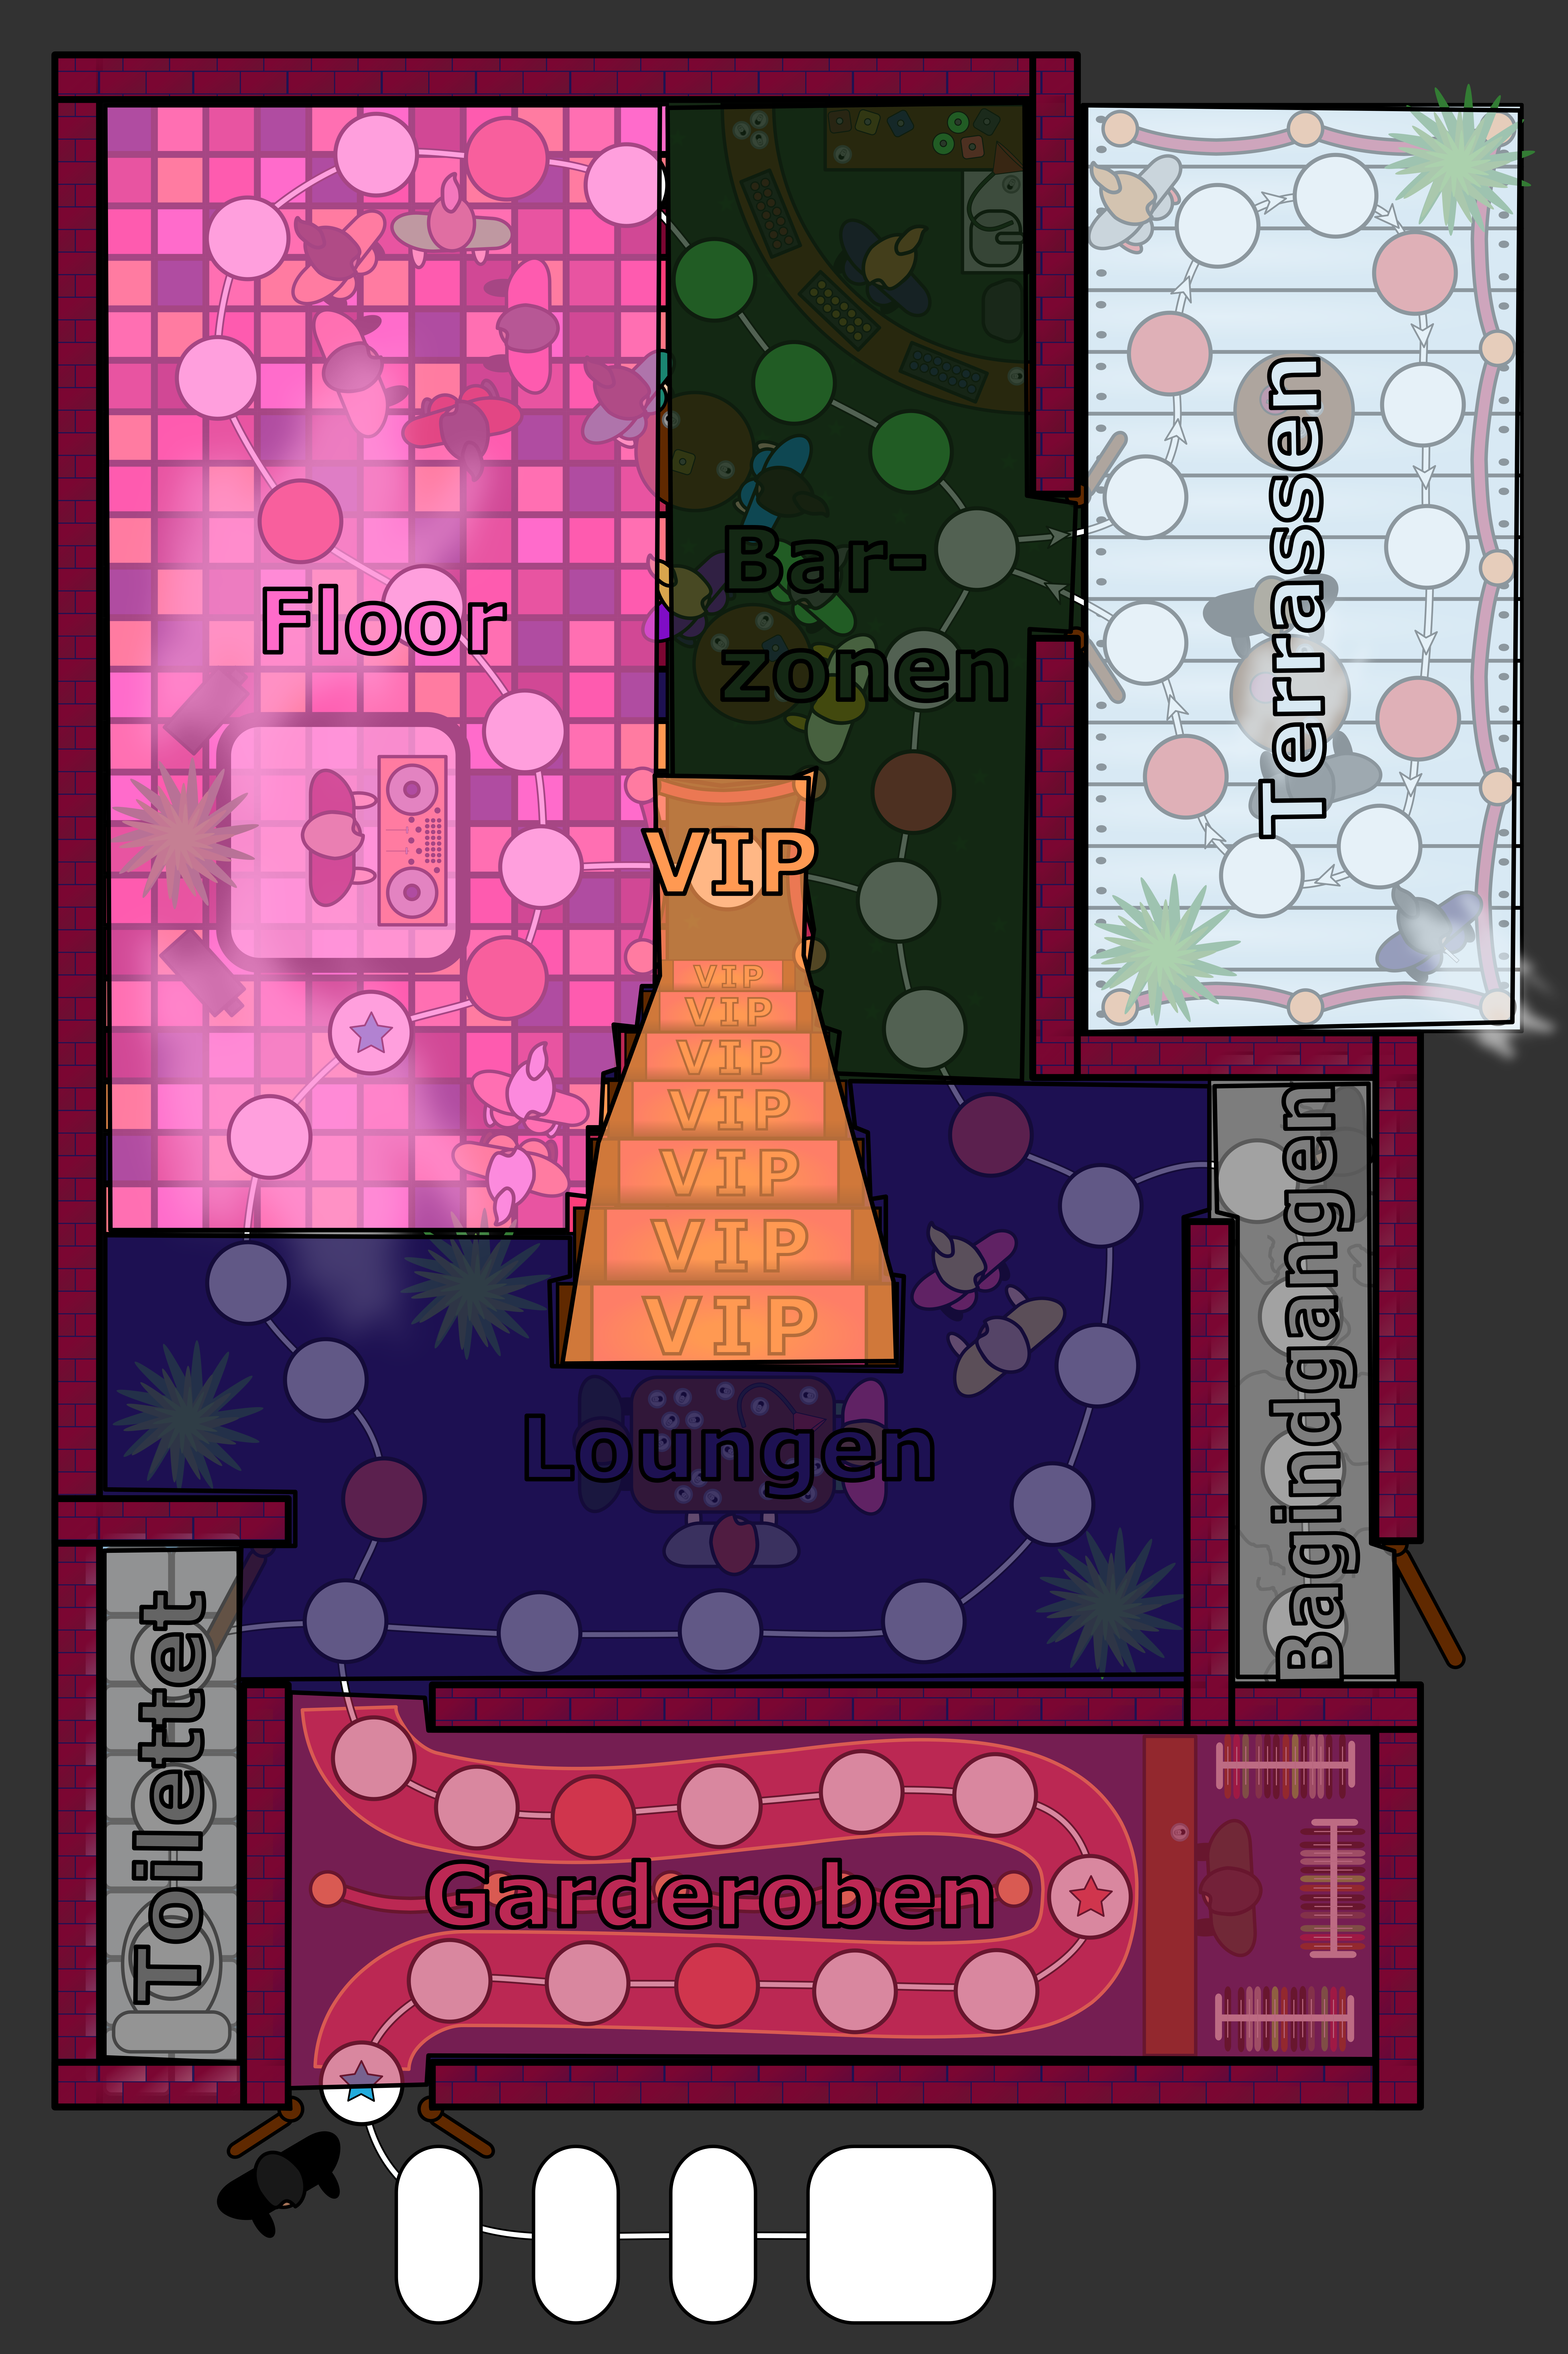
\includegraphics[width=0.9\linewidth]{LeClub_board_zone.png}
\captionof{figure}{Illustration af spillebrættet og zonerne på \LeClub .}
\label{fig:spillebraet}
\end{Figure}

\subsection{Garderoben}
Som en hver anden club har \LeClub\ en garderobe hvor man kan komme af med sit overtøj. Selve garderoben er markeret med en t-shirt der i sig selv er et felt. Det koster 1 pant at komme af med overtøjet. Det er nok bare at passere garderobefeltet for at benytte garderoben. Vælger et hold ikke at betale garderobe for en karakter, bliver karakteren sendt tilbage i garderoben, hvis denne bliver set af dørmanden. 

\subsection{Toilettet}
Har et hold en karakter på toilettet (alle felter i zonen) kan holdet tage en tissepause. Et hold der holder tissepause springes ikke over. Spillet sættes i bero indtil spilleren er tilbage. Toilettet er også det eneste sted der er stille nok til at foretage et telefonopkald. Spillet må generelt ikke forlades uden at man har en karakter på toilettet. Går en spiller fra et hold på toilettet, uden at have en karakter på toilettet først, mister holdets karakter med mest fame alt sit optjente fame. 

Hvis 80\% af alle spillere er enige om at holde en tissepause holdes en tissepause mens spillet er sat i bero. 

\subsection{Bagindgangen}
\hl{Bagindgangen er en utrolig risikabel zone at befinde sig i, men det er her man skal befinde sig for at handle med pusheren (se pusheren).}
Ved bagindgangen kan en karakter lukke karakterer fra samme hold ind uden at de skal betale entre. For at lukke en karakter ind må den anden karakter stå på det yderste felt i bagindgangen. Først må karakteren dog have købt afledningskast i baren (se baren). Før terningekastet kan afledningskastene benyttes (se afledningskast). Rykkes én eller flere karakterer ind som resultat af afledningskastene tæller dette som en tur. En karakter der kommer ind af bagindgangen har ikke stempel på. Heldigvis deler DJ Følerden stempler ud ved hans højre hånd. Det er nok at passere. 

Alle karakterer der bliver set af dørmanden i bagindgangen bliver smidt ud af klubben, med mindre man er venner med dørmanden.

\subsection{Terrassen}
På terrassen er densiteten af røde felter større end i de andre zoner og nogle chancekort kræver tilstedeværelse på terrassen. Man kan kun gå én vej rundt på terrassen. Vejen er anført af pile på spillebrættet. Dørmanden kan ikke være på terrassen. 

\subsection{VIP-loungen}  
Trappen i midten af spillebrættet er VIP-loungen. Feltet inden, indhegnet af røde skillevægge, kan kun betrædes af karakterer, der har optjent nok fame til at komme i VIP-loungen. Hvis en karakter står udenfor VIP-loungen foran en af de røde skillevægge kan man ikke rykke gennem skillevæggen og op i VIP-loungen. Der er spærret.

Når en karakter er gået i VIP-loungen er det ikke muligt at komme tilbage. Karakteren er ude af spillet.  